\documentclass[a4paper, 12pt]{article}
\usepackage[utf8]{inputenc}
\usepackage[lmargin=3cm, tmargin=3cm, rmargin=2cm, bmargin=2cm]{geometry}
\usepackage[onehalfspacing]{setspace}
\usepackage[T1]{fontenc}
\usepackage[brazil]{babel}

%%%\usepackage{amssymb, amsmath, mathptmx}%bigominus

\usepackage{wasysym}%male and female

\usepackage{graphicx, graphics, xcolor, comment, enumerate, multirow, multicol, indentfirst}

\usepackage{amsmath, amsthm, amsfonts, amssymb, dsfont, mathtools}
\everymath{\displaystyle} 

\usepackage{blindtext}

\usepackage[round]{natbib}
\bibliographystyle{apalike}

\usepackage{hyperref}

%Code packages:
\usepackage{listings}
\usepackage{xcolor}

%New colors defined below
\definecolor{codegreen}{rgb}{0,0.6,0}
\definecolor{codegray}{rgb}{0.5,0.5,0.5}
\definecolor{codepurple}{rgb}{0.58,0,0.82}
\definecolor{backcolour}{rgb}{0.95,0.95,0.92}

%Code listing style named "mystyle"
\lstdefinestyle{mystyle}{
  backgroundcolor=\color{backcolour},   commentstyle=\color{codegreen},
  keywordstyle=\color{magenta},
  numberstyle=\tiny\color{codegray},
  stringstyle=\color{codepurple},
  basicstyle=\ttfamily\footnotesize,
  breakatwhitespace=false,         
  breaklines=true,                 
  captionpos=b,                    
  keepspaces=true,                 
  numbers=left,                    
  numbersep=5pt,                  
  showspaces=false,                
  showstringspaces=false,
  showtabs=false,                  
  tabsize=2
}

%"mystyle" code listing set
\lstset{style=mystyle}

\title{Projeto 6: Caos}
\author{
  Herberth Luan Vieira Oliveira\\
  \texttt{12559110}
  \and
  Victor Viana de Oliveira Matos\\
  \texttt{11810821}
  \and
  Vinícius da Costa Collaço\\
  \texttt{11811012}
}

\begin{document}

\maketitle

\section{Introdução}

O trabalho tem objetivo de realizar o uso da técnica vinda da teoria do Caos para decodificação de um código para gerar imagens, com isso testaremos com um arquivo dado em aula e outro enviado de outro grupo da sala. 

\subsection{Sobre a teoria do Caos}
A teoria do Caos é uma área de estudo de matemática que possui diversas aplicações, como sistema dinâmicos. 
O nome Caos no mundo acadêmico aparece por volta dos anos 70, artigo feito por Tien-Yien e James Yorke, com o título de "Período Três Implica Caos".
Tal teoria visa estudar fenômenos que a parecem ser eventos ou possuem dinâmicas aleatórias sem nenhum tipo de ordem , porém quando estudado com maior cautela, percebe-se que há itens que mantém uma periodicidade em meio a visão toda desordenada.
Diante a trabalhos e técnicas desenvolvidas nesse nicho da matemática, o matemático russo Vladimir I. Arnold, desenvolveu uma técnica para transformar algo que não é caótico em caótico que é conhecido como "transformação de do gato de Arnold", modelo matemático que será utilizado para realizar as tarefas deste relatório.

\subsection{A transformação de Arnold}

A transformação de Arnold foi aplicada em uma imagem de um gato, o qual ele foi possível com realizar de uma imagem ordenada em quadrado de dimensões 0,1 deixá-la de maneira totalmente caótica, possuindo uma periodicidade que desse para decodificar e voltar a imagem da maneira que se disponha inicialmente.

O modelo usa técnicas de aritmética modular, que define "se x for um número real mod 1 será único número do intervalo [0,1) que difere de x por um número inteiro. 

  Exemplo: 

            4,2 mod 1 = 0,2  e -3,7 mod 1 = 0,3.

Repare que para números reais não negativos o mod 1 só retornará o valor fracionário de x.
Agora para pares ordenados como (x,y) os valores se comportam como exemplos abaixo:

               (4,2; -3,7) mod = (0,2;0,3)

Na técnica é utilizada um quadro unitário, portanto x mod é um ponto do intervalo [0,1), para qualquer real, deste modo podemos definir:

S = {(x,y)| 0 <= x < 1, 0<= y < 1}

A transformação é definida pela fórmula:

$$\Gamma \left(\begin{bmatrix}
x\\
y
\end{bmatrix}\right)=\begin{bmatrix}
1&1\\
1&2
\end{bmatrix}\begin{bmatrix}
x\\
y
\end{bmatrix}\mathrm{mod\ 1}$$

Para entendimento geométrico da fórmula é necessário uma fatoração:

$$\Gamma \left(\begin{bmatrix}
x\\
y
\end{bmatrix}\right)=\begin{bmatrix}
1&0\\
1&1
\end{bmatrix}\begin{bmatrix}
1&1\\
0&1
\end{bmatrix}\begin{bmatrix}
x\\
y
\end{bmatrix}\mathrm{mod\ 1}$$

Tal fatoração expressa um cisalhamento na direção x de fato 1 e outro de na direção y de mesmo fator, ou seja, a deformação ou deslocamento que a imagem terá na aplicação desta matriz. Importante ressaltar que como estamos utilizando o mod 1, aplicação será feita no quadrado unitário.

A utilização a aplicação do mod 1 é independente do uso após aplicação de uma vez da matriz ou somente no final do processo ou diversas vezes no decorrer do processo, pois a ideia continuará a mesma enquanto a matriz deforma a imagem o mod 1 trará para o quadrante unitário.

Exemplo de procedimento:

Passo 1 - cisalhamento (deslocamento/deformação) em x de fator 1:

$$\begin{bmatrix}
1&1\\
0&1
\end{bmatrix}\begin{bmatrix}
x\\
y
\end{bmatrix} =\begin{bmatrix}
x&+&y\\
&y&
\end{bmatrix}$$

Nesse passo a imagem que estava no quadro unitário começa a se deslocar de maneira horizontalmente a quantidade da tua altura (y).

Passo 2 - cisalhamento (deslocamento/deformação) na direção y de fato 1:

$$\begin{bmatrix}
1&1\\
0&1
\end{bmatrix}\begin{bmatrix}
x\\
y
\end{bmatrix} =\begin{bmatrix}
&x&\\
x&+&y
\end{bmatrix}$$

Nesse passo a imagem que estava deformada de maneira horizontal (eixo x) começa a deformar para vertical no valor da tua abscissa do teu par ordenado.

Finalmente chega-se no passo 3, que é o reagrupamento para o quadro unitário S aplicado o mod 1: (x,y) -> (x,y) mod 1, dimensões [0,1), portanto os pedaços de imagens que foram esticados para além desse limite começam a se deslocar para o quadrado unitário e assim, a imagem começa a deformar e fazendo isso de repetidas vezes a imagem vai se deformando cada vez mais e se tornando um estado caótico.

Desse modo vimos que se criou um cenário caótico devida as repetidas aplicações da matriz ou que podemos nomear de iterações. Essa técnica é conhecida como transformação do gato de Arnold, pois foi realizada iterações numa imagem de um gato e Arnold pelo nome do matemático que desenvolver tal técnica. Mas pontos interessantes foram elencados devido um estudo de 25 iterações realizadas pelo computador com essa técnica:

1 - A posição original volta na 25ª iteração;\\

2 - Em algumas imagens aparecem faixas com sentido específico\\

A explicação do primeiro ponto deve ser considerar algumas premissas antes, primeiro o tratamento da imagem devemos considerar em um plano bidimensional (xy), considerar feixes de cores até 3, ponto é formação da imagem por quadrados discretos chamados de pixels. A exemplo da imagem do gato de Arnold, a imagem possuía uma dimensão 101 x 101, como unidade da imagem é o pixel, então teria o total de 10.201 pixels. Porém o modelo estudado trabalha com dimensões de intervalo de [0,1), então deve-se normalizar a figura, no caso específico dividir as partes por 101, ficando assim (0/101, 1/101, 2/101, 3/101, ..., 101/101). Desta forma os pixels viram pontos de um quadrado unitário, tendo coordenadas de (m/100, n/100), sendo m e n de 0, 1, 2, ..., 100.\\

Podemos generalizar a coordenadas deste plano normalizado dos pontos de pixels p sendo quantidade de pixels de cada lado e as coordenadas: (m/p, n/p), sendo m e n números inteiros de 0 a p - 1.\\

Com essa generalização a transformação de Arnold fica:


$$\Gamma \left(\begin{bmatrix}
m/p\\
n/p
\end{bmatrix}\right)=\begin{bmatrix}
1&1\\
1&2
\end{bmatrix}\begin{bmatrix}
m/p\\
n/p
\end{bmatrix}\mathrm{mod\ 1}=\begin{bmatrix}
(m + n)/p\\
(m + 2n)/p
\end{bmatrix}\mathrm{mod\ 1}$$\\



Com isso o par ordenado toma a forma de ((m+n)/p, (m+2n)/p) é a forma (m'/p, n'/p) o qual m' e n' são tanto o intervalo definido (0 a p-1) e os restantes da divisão de m + n e m + 2n, que são as coordenadas dos pixels para realizar o cisalhamento da figura.\\


A transformação de Arnold possui um plano já definido por S e que tem objetivo de realizar o deslocamento com número máximo de iterações, quando atinge tal ponto dessas iterações o pixel deslocado volta a posição original, mostrando periodicidade que técnica dele admite. Seno variável para número de pixels que imagem detém.\\


Com isso tem-se algumas propriedades a salientar:\\

 - Os pontos eles se movem em n períodos até se retornar ao ponto de partida, logo os pontos são cíclicos e chamado de ciclo do período n;
 
 - pontos como  (0,0) em (0,0) que não só tem o teu n = 1, denotamos como períodos fixos, uma vez, que não mudam de posicionamento depois de n iterações.\\

As fases intermediárias, ou seja, fases que as faixas possuem uma certa orientação específica, mas para explicar podemos ilustrar o exemplo de maneira diferente da aritmética modular e realizar uma leitura da imagem um plano ladrilhado, ou seja, um plano que se tenha vários quadrados unitários S  com a mesma imagem, os quais quando aplicado a transformação de Arnold as imagens começariam a se deslocar e mostrariam uma imagem igual quando se utiliza aritmética modular. Mesmo com o resultado igual, observação importante que a periodicidade tem jeito diferentes de se lidar, enquanto o primeiro modo faz n iterações quando chega ao final do período retornar todos os pixels na tua posição original, o outro modo ao chegar a final de n iterações não retorna na posição original basta pegar os pontos de mesma cor e substituir.

Deste modo temos que pensar que a transformação é linear. Observe a matriz:

$$ C = \begin{bmatrix}
1&1\\
1&2
\end{bmatrix}$$

Ela possui o determinante igual a 1(detalhado no próximo tópico), mas um ponto a ser adiantado que essa propriedade faz com que área multiplicada por essa matriz essa mantida deste modo faz com que os ladrilhos da imagem mantenham a suas proporções consiga fazer a sobreposição de imagem. Portanto, a área de cada iteração continuará a mesma.

A simetria da matriz faz com que os teus autovalores sejam reais e os autovetores correspondentes sejam perpendiculares. Dessa matriz os valores são:

$a1  = \frac{(3 + 5^{\frac{1}{2}})}{2} = 2,6180...\\$


$a2 = \frac{(3 - 5^{\frac{1}{2}})}{2} = 0,3819...\\$

v1 = \begin{bmatrix}
1\\
\frac{(1 + 5^{\frac{1}{2}})}{2}
\end{bmatrix}\\

v2 = \begin{bmatrix}
\frac{(-1 - 5^{\frac{1}{2}})}{2}\\
1
\end{bmatrix}\\

O autovalor a1 faz dilatação na direção do autovetor v1 de fator 2,6180.. enquanto o mesmo acontece na relação de autovalor a2 e v2 diferencia o fator que é 0,3819... .
Como os valores são simétricos os valores começam a centralizar na origem  e de lados paralelos às direções dadas pelos autovetores.
Para explicar as faixas, considere S  como plano ladrilhado e p seja um ponto de S de período n. Como possui um ladrilhamento existe outro ponto q com mesma cor de p, podemos identificar que o ponto $q = (C^{-1})  e p =  C^{-n} p$, pois

$$C^{n} q = C^{n}(C^{-n} p) = p$$

Assim, realizando as iterações sucessivas, os pontos originais se afastam mas ao mesmo tempo outros pontos de mesma cor vão se aproximando dos pontos originais dos teus correspondentes. Essa apresentação mostra que a transformação deixa a imagem caótica mas através de uma orientação que é por esses autovalores e autovetores.


Os pontos de pixels que a transformação de Arnold afeta são valores inteiros, racionais, os pontos racionais são periódico. Inclusive a periodicidade nos pontos é algo essencial para que haja ordem e aplicação dos pixels na transformada. Agora, pode-se existir pontos irracionais em S, os quais não são periódicos, e com isso fazendo as iterações os pontos serão distintos em S. Em teste de computador ter iteradas até 100.000, mostrando os pontos irracionais ficam dispersos, mas com diversas iteradas eles começam a ficar densos em S.
Portanto, podemos concluir que os pontos racionais são densos em S e que após iteradas sucessivas, nem em todos, os pontos irracionais ficam denso em S.\\

Com isso podemos chegar na definição de caos:\\

Uma aplicação T de um conjunto S sobre si mesmo é dita caótica se:\\

(i) S contiver algum conjunto denso de pontos periódicos de T\\

(ii) e existir algum ponto em S cujas iteradas por T são densas em S




\subsection{Sobre as entradas das matrizes chave}
 
As matrizes chaves para a decodificação de uma imagem devem seguir a algumas regras para que a transformação de Arnold funcione como o esperado. em um chave 2x2, cada elemento da matriz deve ter valores positivos e menores que o números de pixel, pois se for maior, o mapeamento pode sair para fora da imagem.

As matrizes também devem ter o \textbf{determinante igual à 1}, pois dessa maneira a transformação \textbf{preserva a área} \citep{9321487} do pixel, em casos que a área é alterada, por menor que seja essa alteração, pode cair em um cenário onde a localização do pixel seja irracional, ou seja, na transformação da imagem m x n, a posição m/p e n/p, seja irracional. Quando temos essa configuração, os pontos irracionais não são periódicos na transformação de Arnold, obtendo assim sempre pontos distintos gerado de um modelo caótico.

Além disso \textbf{os autovalores da matriz chave, devem ter módulos diferentes de 1}, pois a transformação de Arnold caminha no plano da imagem de acordo com os autovalores/autovetores, se o módulo for igual a 1 de algum dos autovalores essa nova localização do pixel, após uma iteração, não irá caminhar para lugar algum, não gerando assim uma transformação cíclica.

\section{Exercício 1}
\subsection{Lendo a imagem}

Abaixo está mostrada a maneira como fizemos a leitura da imagem em \textit{Python}. Supusemos que o arquivo \textit{arnold4\_1.txt} corresponde ao canal de cor vermelho, o arquivo \textit{arnold4\_2.txt} corresponde ao verde, e o \textit{arnold4\_3.txt} ao azul. Explicações detalhadas estão no próprio código.\\

\begin{lstlisting}[language=Python, caption = Lendo dos arquivos .txt e armazenando em estruturas numpy array]
# carregando a imagem em numpy array de duas dimensoes
vermelho = np.loadtxt('../input/dados-map2110-projeto-6-caos/arnold4_1.txt', delimiter='  ')
verde = np.loadtxt('../input/dados-map2110-projeto-6-caos/arnold4_2.txt', delimiter='  ')
azul = np.loadtxt('../input/dados-map2110-projeto-6-caos/arnold4_3.txt', delimiter='   ')

# planificando os arrays para que possamos parear os canais de cor
vermelho_1D = vermelho.flatten()
verde_1D = verde.flatten()
azul_1D = azul.flatten()

# ao parear os canais de cor, retorna-se um array de duas dimensoes
# que porem eh como se fosse linear, pois a segunda dimensao contem apenas os tres canais de cor
imagem_2D = np.array(list(zip(vermelho_1D, verde_1D, azul_1D)))

# É necessario agora colocar o array na forma um "quadrado"(101x101)
imagem_3D = imagem_2D.reshape(101, 101, 3)
\end{lstlisting}

Percebe-se, que da forma como fizemos a leitura dos arquivos para imagem, obtemos uma imagem que está rotacionada 90 no sentido horário, quando comparada com a imagem apresentada no Enunciado do projeto 6, como mostrado abaixo. Utilizamos a biblioteca \textbf{matplotlib.pyplot} importada como \textbf{plt} para plotar o numpy array \textbf{imagem\_3D}:

\begin{center}
    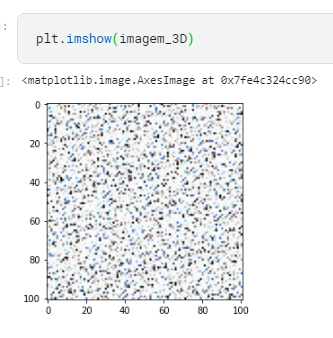
\includegraphics[width=8cm]{01_plot_imagem_3D.PNG}
    
    Imagem Rotacionada 90 graus no sentido horário
\end{center}

Como será visto abaixo, a imagem acima está de acordo com a \textbf{nossa implementação do algoritmo de Arnold}, no qual utilizamos os eixos x e y rotacionados 90 graus no sentido horário, para que fiquem de acordo com a numeração dos índices da linhas e das colunas no \textit{numpy array} que utilizamos para fazer a computação de matrizes. Os eixos x e y da forma padrão para a aplicação do algoritmo de Arnold, bem como a imagem original estão representados na imagem à esquerda abaixo. Já a imagem e os eixos rotacionados representando a forma como nosso algoritmo de Arnold funciona estão representados à direita.

\begin{center}
    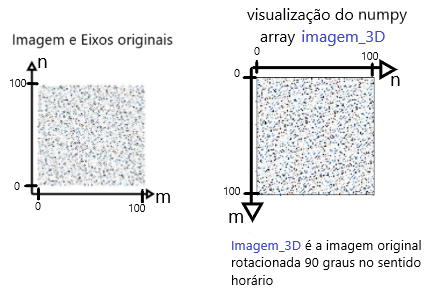
\includegraphics[width=12cm]{02_comparacao_rot.png}
    
    Comparação das imagens sem rotação e com rotação de eixos.
\end{center}

Como evidenciado abaixo, o numpy array \textbf{imagem\_3D} já pode ser aplicado sem problemas em nosso algoritmo, pois os índices aqui utilizados nas computações com matrizes assumem a forma rotacionada de noventa graus no sentido horário.
Porém, todas as imagens resultados das aplicações da transformação de Arnold também estarão rotacionadas de 90 graus no sentido horário.

Se quisermos ver a imagem na orientação correta, basta que apenas nos momentos de visualizar as imagens se rotacione 90 graus no sentido \textbf{anti-horário}.

\subsection{Algoritmo de Arnold}

Para este exercício a transformação de Arnold que utilizamos é da seguinte forma \citep{anton}:

$$\Gamma \left(\begin{bmatrix}
m/p\\
n/p
\end{bmatrix}\right)=\begin{bmatrix}
1&1\\
1&2
\end{bmatrix}\begin{bmatrix}
m/p\\
n/p
\end{bmatrix}\mathrm{mod\ 1}$$

Em que $p = 101$, já que a imagem tem dimensões de 101x101. E $m$ e $n$ são número inteiros no intervalo $[0, 100]$.

Para a criação do algoritmo de Arnold, implementado em python, o algoritmo foi desenvolvido de modo que é possível entrar com qualquer tamanho de imagem quadrada. A medida do tamanho dos pixels é feita pelo método shape da biblioteca Numpy.

\begin{lstlisting}[language=Python, caption = Algoritmo de Arnold]
def arnold(img, matriz_chave=np.array([[1, 1],[1, 2]]), it=30):
  n_pixel = img.shape[0]
  nova_img = np.zeros(img.shape)

  #criacao da figura, subplots com 5 colunas
  fig = plt.figure(figsize=(100, 120))
  plot_columns = 5
  plot_rows = int(it/plot_columns)

  for i in range(it):
    for m in range(n_pixel):
      for n in range(n_pixel):
        pixel = np.array([[m], [n]])
        nova_pos = (matriz_chave @ pixel/n_pixel)%1
        nova_pos *= n_pixel
        novo_m = int((nova_pos[0]).round())
        novo_n = int((nova_pos[1]).round())
        nova_img[novo_m][novo_n] = img[m][n]

    #cada iteracao em um subplot
    fig.add_subplot(plot_rows, plot_columns, i+1)
    plt.imshow(img)
    plt.axis('off')

    #necessario criar um copia para funcionar
    img = np.copy(nova_img)

    #Salvar uma das iteracoes para o outro grupo
    if i == 6:
      img_grupo = np.copy(img)
  return img_grupo
\end{lstlisting}

O algoritmo aplica a transformação de Arnold para uma imagem quadrada, reorganizando os pixels de acordo com a chave de entrada e a cada iteração e mostrando a imagem gerada em um subplot a cada iteração. Após a multiplicação matricial e cálculo do módulo, foi necessário arredondar os valores para inteiros, para que mapeasse a imagem de forma correta.

No final do algoritmo foi retornado uma das iterações para futuro envio da nossa imagem decodificada para um outro grupo.

\subsection{Decodificando a imagem}

Finalmente, usando o algoritmo de Arnold definido acima e passando como parâmetro o numpy array \textbf{imagem\_3D}, conseguimos decodificar a imagem dada, na iteração de número 20. Foi utilizado a matriz [[1, 1], [1, 2]] definida como padrão, e 30 iterações, como está mostrado abaixo:

\begin{lstlisting}[language=Python, caption=Chamando a função arnold para a imagem_3D]
arnold(imagem_3D, it=30)

\end{lstlisting}

\begin{center}
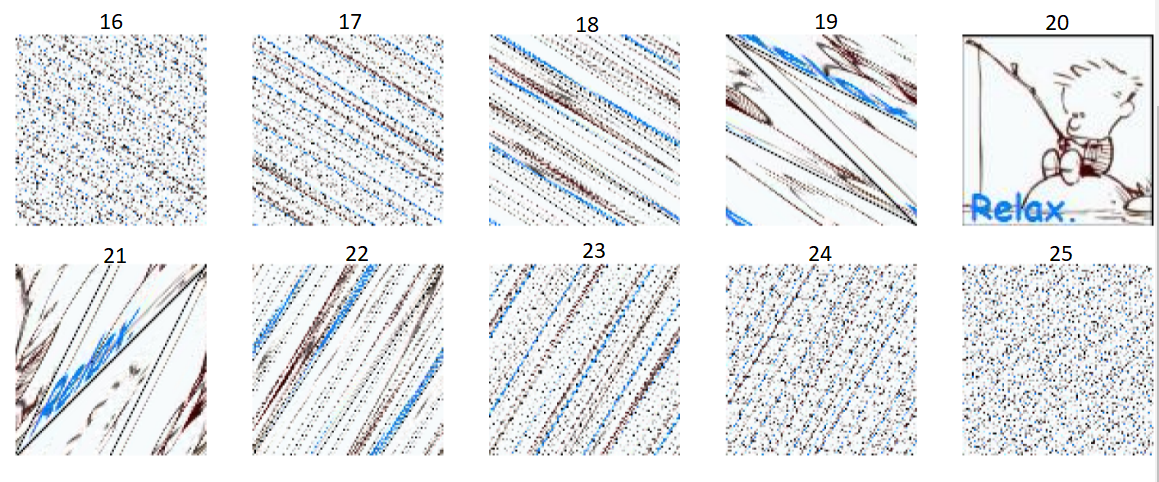
\includegraphics[width=16cm]{Relax_01.PNG}

Saída da função arnold: Iterações de 16 a 25 do processo de decodificação.
\end{center}

Portanto a imagem decodificada é:

\begin{center}

\includegraphics[width=8cm]{Relax.PNG}

Imagem decodificada.
\end{center}


\section{Exercício 2}
O grupo com o qual escolhemos trabalhar tem os seguintes integrantes:

\begin{itemize}
    \item Danton Takashi Fukuda Koga (12557762)
    \item Isaac Cavalcante Ferreira (12558613)
    \item José Luiz Silva Ramos Cavalcanti (12557056)
    \item Pedro Akira Kitayama (11271907)
    \item Vitor Martins Santos (11261955)
\end{itemize}

\subsection{Preparando a imagem para o outro grupo}

A arte da imagem escolhida para ser decodificada pelo o outro grupo, foi feita digitalmente à mão livre. Foi inicialmente feita para teste do algoritmo de Arnold, mas foi mantida por ter um desenho mais simplificado, de fácil reconhecimento. 

\begin{center}

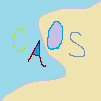
\includegraphics[width=8cm]{Caos.png}

Imagem para ser decodificada

\end{center}

Para a decodificação para o outro grupo foi utilizada a chave $\begin{bmatrix} 1 & 6 \\ 2 & 13\end{bmatrix}$ para gerar a imagem codificada foi utilizado a mesma função "arnold", retornando na 6 iteração.

Com a chave utilizada, uma imagem de 101x101 pixels, tem ciclo de 17 iterações, ou seja, a cada 17 iterações a imagem se repete.

\begin{lstlisting}[language=Python, caption=Imagem Codificada]
matriz_chave = np.array([[1, 6], [2, 13]])
it = 25
imagem_grupo = arnold2(caos_norm, matriz_chave, it)
\end{lstlisting}

\begin{center}
    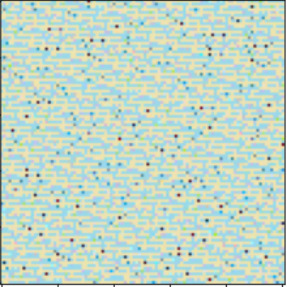
\includegraphics[width=8cm]{imagem_grupo.jpg}
    
    imagem codificada enviada para o outro grupo
\end{center}
A imagem decodificada foi armazenada na variável imagem\_grupo, e para transformar cada cor em um arquivo texto foi utilizado o método savetxt da biblioteca Numpy, com o seguinte código:

\begin{lstlisting}[language=Python, caption=imagem codificada para texto]
np.savetxt('Imagem_grupo_r.txt',imagem_grupo[:,:,0], delimiter=' ')
np.savetxt('Imagem_grupo_g.txt',imagem_grupo[:,:,1], delimiter=' ')
np.savetxt('Imagem_grupo_b.txt',imagem_grupo[:,:,2], delimiter=' ')
\end{lstlisting}

Então após esses processos, foram enviados para o outro grupo os três arquivos textos e a imagem decodificada de referência.

\subsection{Decodificando a imagem do outro grupo}


\subsubsection{Leitura dos arquivos}

Recebemos do outro grupo, 3 arquivos .txt como os seguintes nomes: \textbf{b1.txt}, \textbf{b2.txt} e \textbf{b3.txt}, cada um dos quais representando, respectivamente, os canais de cor \textbf{vermelho}, \textbf{verde} e \textbf{azul}.

Então, prosseguimos para a leitura desses arquivos para estruturas \textit{numpy array}, e manipulamos estes arrays para juntar todos os canais de de cor em um único array, como feito no exercício 1. O procedimento descrito é retratado em código abaixo:

\begin{lstlisting}[language=Python, caption = Lendo dos arquivos .txt e armazenando em estruturas numpy array ]
red_them = np.loadtxt('../input/d/victorvianaom/dados-map2110-projeto-6-caos/b1.txt', delimiter=' ')
green_them = np.loadtxt('../input/d/victorvianaom/dados-map2110-projeto-6-caos/b2.txt', delimiter=' ')
blue_them = np.loadtxt('../input/d/victorvianaom/dados-map2110-projeto-6-caos/b3.txt', delimiter=' ')

red_them_1D = red_them.flatten()
green_them_1D = green_them.flatten()
blue_them_1D = blue_them.flatten()

image_them_2D = np.array(list(zip(red_them_1D, green_them_1D, blue_them_1D)))
image_them_3D = image_them_2D.reshape(101, 101, 3)
\end{lstlisting}

Portando, a imagem codificada do outro grupo está armazenada no numpy array \textbf{image\_them\_3D}. Visualizando este objeto através do comando abaixo temos a seguinte imagem:

\begin{center}
    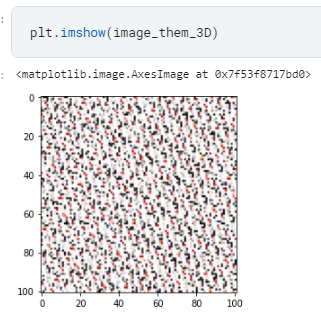
\includegraphics[width=8cm]{03_image_them_plot.PNG}
    
    Imagem codificada recebida.
\end{center}

\subsubsection{Calculando todas as matrizes chave possíveis}

Como visto na introdução, as matrizes chave são da seguinte forma:

$$\mathrm{C}=\begin{bmatrix}
a&b\\
c&d
\end{bmatrix}$$

Submetidas as restrições:

\begin{itemize}
    \item Pode-se restringir os valores de a,b,c e d ao intervalo $[0, 100]$;
    \item O determinante de $\mathrm{C}$ deve ser igual a 1. Isto é: $ad-bc=1$;
    \item $\mathrm{C}$ não pode ter nenhum autovalor com módulo igual a 1.
\end{itemize}

Programando em Python as restrições acima tem-se:\\

\begin{lstlisting}[language=Python, caption = Filtrando valores com base nas restrições]
# Verificando valores de a,b,c e tais que o determinante de [[a, b], [c, d]] e igual a 1
possiveis_det = []
for a in range(101):
  for b in range(101):
    for c in range(101):
      for d in range(101):
        if (a*d - b*c) == 1:
          possiveis_det.append([[a, b], [c, d]])

# Dos resultados encontrados acima, considera-se abaixo apenas aqueles em que
# nao se tem nenhum autovalor com modulo igual a 1
possiveis_det_autovalores = []

for matriz in possiveis_det:
  if 1 not in abs(np.linalg.eig(matriz)[0]):
    possiveis_det_autovalores.append(matriz)
\end{lstlisting}

Portanto, agora a lista \textbf{possiveis\_det\_autovalores} possui todas as possibilidades para a matriz chave. São 11.974 possibilidades como visto abaixo:

\begin{center}
    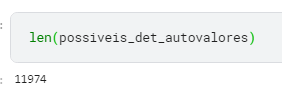
\includegraphics[width=8cm]{04_len_possiveis_det_autovalores.PNG}
    
    Quantidades de matrizes chave possíveis.
\end{center}

\subsubsection{Ordenando pelos menores valores da soma a+b+c+d}

Partindo da suposição de que o outro grupo não escolheu uma matriz chave com valores muito grandes, colocamos as matrizes da lista \textbf{possiveis\_det\_autovalores} em ordem crescente da soma $a+b+c+d$.

Abaixo está a implementação em Python desta premissa:

\begin{lstlisting}[language=Python, caption = Colocando em ordem crescente da soma a+b+c+d]
sum_abcd = []

for i in range(len(possiveis_det_autovalores)):
    sum_abcd.append([i, np.sum(possiveis_det_autovalores[i])])

sorted_sum_abcd = sorted(sum_abcd, key=lambda x: x[1])
\end{lstlisting}

Podemos ver que \textbf{sorted\_sum\_abcd[i][0]} representa o índice da lista\\ \textbf{possiveis\_det\_autovalores} de forma ordenada. Mostrando os 10 primeiros índices ordenados pela soma tem-se as seguintes matrizes chave:

\begin{center}
    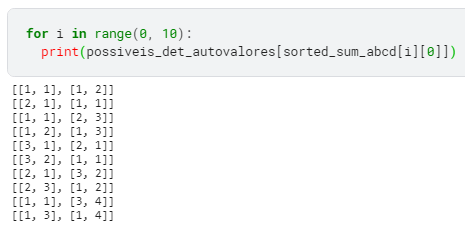
\includegraphics[width=12cm]{05_10_primeiros_sorted.PNG}
    
    Primeiras 10 chaves da lista possiveis\_det\_autovalores ordenados.
\end{center}

\subsubsection{Tentativas, Fracassos e Resultados Interessantes}

Nós utilizamos de \textbf{força-bruta}, tentando as chaves na ordem crescente da soma a+b+c+d, até que possivelmente encontrássemos o resultado. Cada tentativa for feita manualmente, executando em blocos de 20, com 20 células de um Jupyter Notebook do Google Colab (por vezes também utilizamos os Notebooks do Kaggle), executando uma após a outra. Enquanto verificávamos visualmente se as imagens retornadas tinham um padrão, outra célula executava e assim por diante.

Num primeiro momento, nós não nos atentamos para a quantidade de iterações e deixamos fixada em 30, como no exercício 1, em todas as tentativas.

Então tentamos para todas as 351 primeiras chaves, que são as seguintes:

\begin{lstlisting}[language=Python, caption = 351 chaves tentadas num primeiro momento.]
for i in range(0, 350):
  print(possiveis_det_autovalores[sorted_sum_abcd[i][0]], ', ', end='')
\end{lstlisting}

\begin{footnotesize}
[[1, 1], [1, 2]] , [[2, 1], [1, 1]] , [[1, 1], [2, 3]] , [[1, 2], [1, 3]] , [[3, 1], [2, 1]] , [[3, 2], [1, 1]] , [[2, 1], [3, 2]] , [[2, 3], [1, 2]] , [[1, 1], [3, 4]] , [[1, 3], [1, 4]] , [[4, 1], [3, 1]] , [[4, 3], [1, 1]] , [[1, 2], [2, 5]] , [[5, 2], [2, 1]] , [[1, 1], [4, 5]] , [[1, 4], [1, 5]] , [[2, 1], [5, 3]] , [[2, 5], [1, 3]] , [[3, 1], [5, 2]] , [[3, 5], [1, 2]] , [[5, 1], [4, 1]] , [[5, 4], [1, 1]] , [[3, 2], [4, 3]] , [[3, 4], [2, 3]] , [[1, 1], [5, 6]] , [[1, 2], [3, 7]] , [[1, 3], [2, 7]] , [[1, 5], [1, 6]] , [[2, 3], [3, 5]] , [[5, 3], [3, 2]] , [[6, 1], [5, 1]] , [[6, 5], [1, 1]] , [[7, 2], [3, 1]] , [[7, 3], [2, 1]] , [[2, 1], [7, 4]] , [[2, 7], [1, 4]] , [[4, 1], [7, 2]] , [[4, 7], [1, 2]] , [[1, 1], [6, 7]] , [[1, 6], [1, 7]] , [[3, 1], [8, 3]] , [[3, 8], [1, 3]] , [[7, 1], [6, 1]] , [[7, 6], [1, 1]] , [[1, 2], [4, 9]] , [[1, 4], [2, 9]] , [[4, 3], [5, 4]] , [[4, 5], [3, 4]] , [[9, 2], [4, 1]] , [[9, 4], [2, 1]] , [[1, 1], [7, 8]] , [[1, 3], [3, 10]] , [[1, 7], [1, 8]] , [[2, 1], [9, 5]] , [[2, 9], [1, 5]] , [[3, 2], [7, 5]] , [[3, 7], [2, 5]] , [[5, 1], [9, 2]] , [[5, 2], [7, 3]] , [[5, 7], [2, 3]] , [[5, 9], [1, 2]] , [[8, 1], [7, 1]] , [[8, 7], [1, 1]] , [[10, 3], [3, 1]] , [[2, 3], [5, 8]] , [[2, 5], [3, 8]] , [[8, 3], [5, 2]] , [[8, 5], [3, 2]] , [[1, 1], [8, 9]] , [[1, 2], [5, 11]] , [[1, 5], [2, 11]] , [[1, 8], [1, 9]] , [[3, 1], [11, 4]] , [[3, 4], [5, 7]] , [[3, 5], [4, 7]] , [[3, 11], [1, 4]] , [[4, 1], [11, 3]] , [[4, 11], [1, 3]] , [[7, 4], [5, 3]] , [[7, 5], [4, 3]] , [[9, 1], [8, 1]] , [[9, 8], [1, 1]] , [[11, 2], [5, 1]] , [[11, 5], [2, 1]] , [[2, 1], [11, 6]] , [[2, 11], [1, 6]] , [[5, 4], [6, 5]] , [[5, 6], [4, 5]] , [[6, 1], [11, 2]] , [[6, 11], [1, 2]] , [[1, 1], [9, 10]] , [[1, 3], [4, 13]] , [[1, 4], [3, 13]] , [[1, 9], [1, 10]] , [[5, 3], [8, 5]] , [[5, 8], [3, 5]] , [[10, 1], [9, 1]] , [[10, 9], [1, 1]] , [[13, 3], [4, 1]] , [[13, 4], [3, 1]] , [[1, 2], [6, 13]] , [[1, 6], [2, 13]] , [[3, 2], [10, 7]] , [[3, 10], [2, 7]] , [[7, 2], [10, 3]] , [[7, 10], [2, 3]] , [[13, 2], [6, 1]] , [[13, 6], [2, 1]] , [[1, 1], [10, 11]] , [[1, 10], [1, 11]] , [[2, 1], [13, 7]] , [[2, 3], [7, 11]] , [[2, 7], [3, 11]] , [[2, 13], [1, 7]] , [[3, 1], [14, 5]] , [[3, 14], [1, 5]] , [[4, 3], [9, 7]] , [[4, 9], [3, 7]] , [[5, 1], [14, 3]] , [[5, 14], [1, 3]] , [[7, 1], [13, 2]] , [[7, 3], [9, 4]] , [[7, 9], [3, 4]] , [[7, 13], [1, 2]] , [[11, 1], [10, 1]] , [[11, 3], [7, 2]] , [[11, 7], [3, 2]] , [[11, 10], [1, 1]] , [[4, 1], [15, 4]] , [[4, 15], [1, 4]] , [[5, 2], [12, 5]] , [[5, 12], [2, 5]] , [[6, 5], [7, 6]] , [[6, 7], [5, 6]] , [[1, 1], [11, 12]] , [[1, 2], [7, 15]] , [[1, 3], [5, 16]] , [[1, 5], [3, 16]] , [[1, 7], [2, 15]] , [[1, 11], [1, 12]] , [[2, 5], [5, 13]] , [[4, 5], [7, 9]] , [[4, 7], [5, 9]] , [[9, 5], [7, 4]] , [[9, 7], [5, 4]] , [[12, 1], [11, 1]] , [[12, 11], [1, 1]] , [[13, 5], [5, 2]] , [[15, 2], [7, 1]] , [[15, 7], [2, 1]] , [[16, 3], [5, 1]] , [[16, 5], [3, 1]] , [[1, 4], [4, 17]] , [[2, 1], [15, 8]] , [[2, 15], [1, 8]] , [[3, 4], [8, 11]] , [[3, 8], [4, 11]] , [[8, 1], [15, 2]] , [[8, 15], [1, 2]] , [[11, 4], [8, 3]] , [[11, 8], [4, 3]] , [[17, 4], [4, 1]] , [[1, 1], [12, 13]] , [[1, 12], [1, 13]] , [[3, 1], [17, 6]] , [[3, 2], [13, 9]] , [[3, 5], [7, 12]] , [[3, 7], [5, 12]] , [[3, 13], [2, 9]] , [[3, 17], [1, 6]] , [[6, 1], [17, 3]] , [[6, 17], [1, 3]] , [[9, 2], [13, 3]] , [[9, 13], [2, 3]] , [[12, 5], [7, 3]] , [[12, 7], [5, 3]] , [[13, 1], [12, 1]] , [[13, 12], [1, 1]] , [[1, 2], [8, 17]] , [[1, 8], [2, 17]] , [[2, 3], [9, 14]] , [[2, 9], [3, 14]] , [[7, 6], [8, 7]] , [[7, 8], [6, 7]] , [[14, 3], [9, 2]] , [[14, 9], [3, 2]] , [[17, 2], [8, 1]] , [[17, 8], [2, 1]] , [[1, 1], [13, 14]] , [[1, 3], [6, 19]] , [[1, 6], [3, 19]] , [[1, 13], [1, 14]] , [[2, 1], [17, 9]] , [[2, 17], [1, 9]] , [[4, 1], [19, 5]] , [[4, 19], [1, 5]] , [[5, 1], [19, 4]] , [[5, 3], [13, 8]] , [[5, 4], [11, 9]] , [[5, 7], [7, 10]] , [[5, 11], [4, 9]] , [[5, 13], [3, 8]] , [[5, 19], [1, 4]] , [[8, 3], [13, 5]] , [[8, 13], [3, 5]] , [[9, 1], [17, 2]] , [[9, 4], [11, 5]] , [[9, 11], [4, 5]] , [[9, 17], [1, 2]] , [[10, 7], [7, 5]] , [[14, 1], [13, 1]] , [[14, 13], [1, 1]] , [[19, 3], [6, 1]] , [[19, 6], [3, 1]] , [[4, 3], [13, 10]] , [[4, 13], [3, 10]] , [[7, 4], [12, 7]] , [[7, 12], [4, 7]] , [[10, 3], [13, 4]] , [[10, 13], [3, 4]] , [[1, 1], [14, 15]] , [[1, 2], [9, 19]] , [[1, 4], [5, 21]] , [[1, 5], [4, 21]] , [[1, 9], [2, 19]] , [[1, 14], [1, 15]] , [[3, 1], [20, 7]] , [[3, 20], [1, 7]] , [[5, 2], [17, 7]] , [[5, 6], [9, 11]] , [[5, 9], [6, 11]] , [[5, 17], [2, 7]] , [[7, 1], [20, 3]] , [[7, 2], [17, 5]] , [[7, 5], [11, 8]] , [[7, 11], [5, 8]] , [[7, 17], [2, 5]] , [[7, 20], [1, 3]] , [[8, 5], [11, 7]] , [[8, 11], [5, 7]] , [[11, 6], [9, 5]] , [[11, 9], [6, 5]] , [[15, 1], [14, 1]] , [[15, 14], [1, 1]] , [[19, 2], [9, 1]] , [[19, 9], [2, 1]] , [[21, 4], [5, 1]] , [[21, 5], [4, 1]] , [[2, 1], [19, 10]] , [[2, 5], [7, 18]] , [[2, 7], [5, 18]] , [[2, 19], [1, 10]] , [[3, 2], [16, 11]] , [[3, 16], [2, 11]] , [[8, 7], [9, 8]] , [[8, 9], [7, 8]] , [[10, 1], [19, 2]] , [[10, 19], [1, 2]] , [[11, 2], [16, 3]] , [[11, 16], [2, 3]] , [[18, 5], [7, 2]] , [[18, 7], [5, 2]] , [[1, 1], [15, 16]] , [[1, 3], [7, 22]] , [[1, 7], [3, 22]] , [[1, 15], [1, 16]] , [[2, 3], [11, 17]] , [[2, 11], [3, 17]] , [[3, 4], [11, 15]] , [[3, 11], [4, 15]] , [[7, 3], [16, 7]] , [[7, 16], [3, 7]] , [[15, 4], [11, 3]] , [[15, 11], [4, 3]] , [[16, 1], [15, 1]] , [[16, 15], [1, 1]] , [[17, 3], [11, 2]] , [[17, 11], [3, 2]] , [[22, 3], [7, 1]] , [[22, 7], [3, 1]] , [[1, 2], [10, 21]] , [[1, 10], [2, 21]] , [[4, 1], [23, 6]] , [[4, 5], [11, 14]] , [[4, 11], [5, 14]] , [[4, 23], [1, 6]] , [[5, 8], [8, 13]] , [[6, 1], [23, 4]] , [[6, 23], [1, 4]] , [[13, 8], [8, 5]] , [[14, 5], [11, 4]] , [[14, 11], [5, 4]] , [[21, 2], [10, 1]] , [[21, 10], [2, 1]] , [[1, 1], [16, 17]] , [[1, 16], [1, 17]] , [[2, 1], [21, 11]] , [[2, 21], [1, 11]] , [[3, 1], [23, 8]] , [[3, 5], [10, 17]] , [[3, 10], [5, 17]] , [[3, 23], [1, 8]] , [[5, 1], [24, 5]] , [[5, 24], [1, 5]] , [[6, 5], [13, 11]] , [[6, 13], [5, 11]] , [[8, 1], [23, 3]] , [[8, 23], [1, 3]] , [[11, 1], [21, 2]] , [[11, 5], [13, 6]] , [[11, 13], [5, 6]] , [[11, 21], [1, 2]] , [[17, 1], [16, 1]] , [[17, 5], [10, 3]] , [[17, 10], [5, 3]] , [[17, 16], [1, 1]] , [[1, 4], [6, 25]] , [[1, 6], [4, 25]] , [[4, 7], [9, 16]] , [[4, 9], [7, 16]] , [[9, 8], [10, 9]] , [[9, 10], [8, 9]] , [[16, 7], [9, 4]] , [[16, 9], [7, 4]] , [[25, 4], [6, 1]] , [[25, 6], [4, 1]] , [[1, 1], [17, 18]] , [[1, 2], [11, 23]] , [[1, 3], [8, 25]] , [[1, 5], [5, 26]] , [[1, 8], [3, 25]] , [[1, 11], [2, 23]] , [[1, 17], [1, 18]] , [[3, 2], [19, 13]] , [[3, 7], [8, 19]] , [[3, 8], [7, 19]] , [[3, 19], [2, 13]] , [[4, 3], [17, 13]] , [[4, 17], [3, 13]] , [[5, 3], [18, 11]] , [[5, 18], [3, 11]] , [[6, 7], [11, 13]] , [[6, 11], [7, 13]] , [[11, 3], [18, 5]] , [[11, 18], [3, 5]] , [[13, 2], [19, 3]] , [[13, 3], [17, 4]] , [[13, 7], [11, 6]] , [[13, 11], [7, 6]] , [[13, 17], [3, 4]]
\end{footnotesize}\\

A chamada para a função que define o algoritmo de Arnold, foi feita da seguinte forma padrão, em que i representa cada uma das tentativas. Porém não colocamos em um loop padrão do Python, nós mudamos os valores de i manualmente:

\begin{lstlisting}[language=Python, caption = chamada do algoritmo de Arnold.]
i = 350
arnold(image_them_3D, possiveis_det_autovalores[sorted_sum_abcd[i][0]], it=30)
\end{lstlisting}

Não obtivemos sucesso com nenhuma dessas chaves, mais tarde descobrimos que na realidade já havíamos testado a matriz chave correta, e que bastaria aumentar a quantidade de iterações para que a imagem decodificada aparecesse.

Porém, alguns resultados interessantes apareceram com essas tentativas, que são elas: \\

\textbf{Para a chave [[6, 5], [7, 6]], chegamos a encontrar a seguinte imagem}:

\begin{center}
    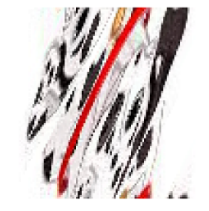
\includegraphics[width=8cm]{132.PNG}
    
    Imagem encontrada em uma das iterações da chave [[6, 5], [7, 6]].
\end{center}
$$$$\\\\\\\\\\\\\\

\textbf{Usando a chave [[19, 2], [9, 1]] é possível obter a imagem:}

\begin{center}
    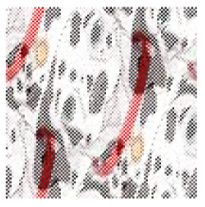
\includegraphics[width=8cm]{244.PNG}
    
    Padrão obtido: chave [[19, 2], [9, 1]].
\end{center}

\textbf{E com a chave [[1, 8], [3, 25]] obtemos o seguinte padrão}

\begin{center}
    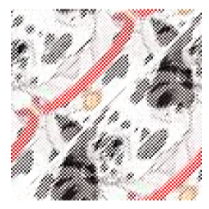
\includegraphics[width=8cm]{330.PNG}
    
    Padrão obtido: chave [[1, 8], [3, 25]].
\end{center}

A partir deste ponto sabíamos que a imagem decodificada representava um \textbf{cachorro}, faltava apenas encontrar a chave correta.

Foi então que decidimos aumentar o número de iterações para 150 e tivemos sucesso como será mostrado a seguir.

\subsubsection{Decodificando a imagem com Sucesso}

Então, como já tínhamos tentado pra diversas matrizes chave sem sucesso decidimos aumentar o número de iterações para 150, um valor arbitrário, mas suficientemente alto para que aumente as chances de a imagem se mostrar decodificada.

Neste esquema tentamos para os índices \textbf{sorted\_sum\_abcd[i][0]}, para i indo de 0 a 67. Até que quando $i=67$ nós conseguimos decodificar a imagem.

Neste caso, as 68 matrizes chave testadas foram:

\begin{lstlisting}[language=Python, caption = chamada do algorítimo de Arnold.]
for i in range(0, 67):
  print(possiveis_det_autovalores[sorted_sum_abcd[i][0]], ', ', end='')
\end{lstlisting}

\begin{footnotesize}
[[1, 1], [1, 2]] , [[2, 1], [1, 1]] , [[1, 1], [2, 3]] , [[1, 2], [1, 3]] , [[3, 1], [2, 1]] , [[3, 2], [1, 1]] , [[2, 1], [3, 2]] , [[2, 3], [1, 2]] , [[1, 1], [3, 4]] , [[1, 3], [1, 4]] , [[4, 1], [3, 1]] , [[4, 3], [1, 1]] , [[1, 2], [2, 5]] , [[5, 2], [2, 1]] , [[1, 1], [4, 5]] , [[1, 4], [1, 5]] , [[2, 1], [5, 3]] , [[2, 5], [1, 3]] , [[3, 1], [5, 2]] , [[3, 5], [1, 2]] , [[5, 1], [4, 1]] , [[5, 4], [1, 1]] , [[3, 2], [4, 3]] , [[3, 4], [2, 3]] , [[1, 1], [5, 6]] , [[1, 2], [3, 7]] , [[1, 3], [2, 7]] , [[1, 5], [1, 6]] , [[2, 3], [3, 5]] , [[5, 3], [3, 2]] , [[6, 1], [5, 1]] , [[6, 5], [1, 1]] , [[7, 2], [3, 1]] , [[7, 3], [2, 1]] , [[2, 1], [7, 4]] , [[2, 7], [1, 4]] , [[4, 1], [7, 2]] , [[4, 7], [1, 2]] , [[1, 1], [6, 7]] , [[1, 6], [1, 7]] , [[3, 1], [8, 3]] , [[3, 8], [1, 3]] , [[7, 1], [6, 1]] , [[7, 6], [1, 1]] , [[1, 2], [4, 9]] , [[1, 4], [2, 9]] , [[4, 3], [5, 4]] , [[4, 5], [3, 4]] , [[9, 2], [4, 1]] , [[9, 4], [2, 1]] , [[1, 1], [7, 8]] , [[1, 3], [3, 10]] , [[1, 7], [1, 8]] , [[2, 1], [9, 5]] , [[2, 9], [1, 5]] , [[3, 2], [7, 5]] , [[3, 7], [2, 5]] , [[5, 1], [9, 2]] , [[5, 2], [7, 3]] , [[5, 7], [2, 3]] , [[5, 9], [1, 2]] , [[8, 1], [7, 1]] , [[8, 7], [1, 1]] , [[10, 3], [3, 1]] , [[2, 3], [5, 8]] , [[2, 5], [3, 8]] , [[8, 3], [5, 2]]
\end{footnotesize}\\

Chamamos manualmente a função que define o algoritmo de Arnold, até que i=67, como mostrado abaixo:

\begin{lstlisting}[language=Python, caption = chamada do algorítimo de Arnold.]
i = 67
arnold(image_them_3D, possiveis_det_autovalores[sorted_sum_abcd[i][0]], it=150)

\end{lstlisting}

\begin{center}
    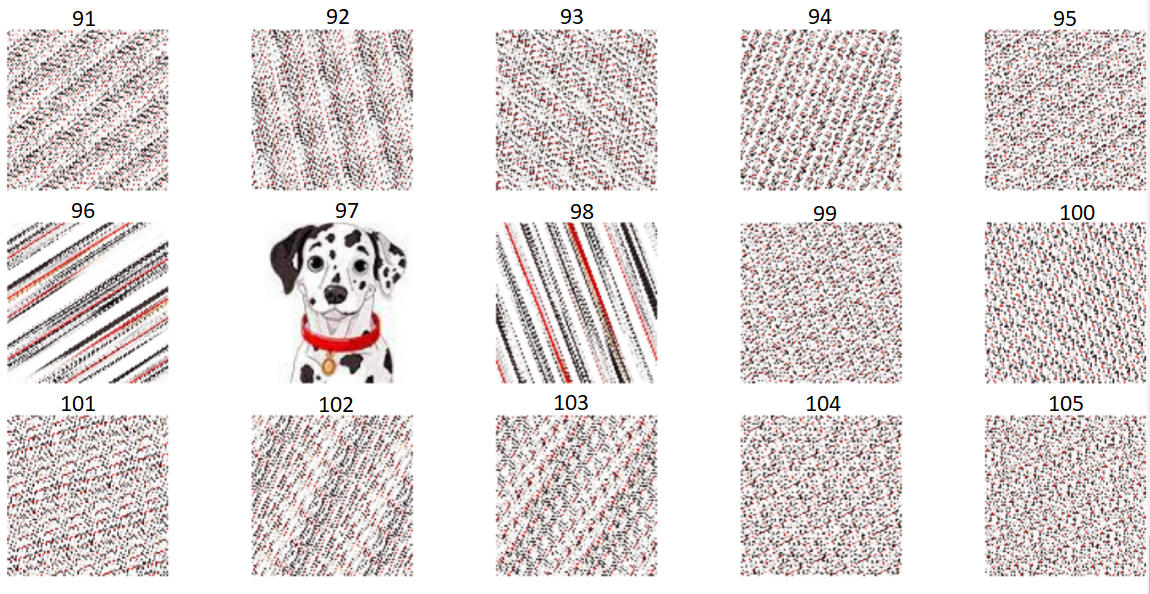
\includegraphics[width=16cm]{ihuuu_01.PNG}
    
    Saída da função arnold: Iterações de 91 a 105 usando a chave [[8, 5], [3, 2]].
\end{center}

A imagem que apareceu decodificada na iteração 97 da tentativa 67 é:

\begin{center}
    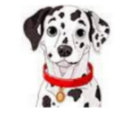
\includegraphics[width=8cm]{ihuuu.PNG}
    
    Imagem decodificada.
\end{center}


Temos que quando i=67 a matriz-chave resposta é dada por:

\begin{center}
    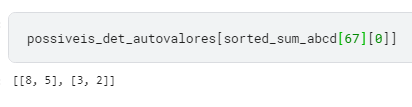
\includegraphics[width=12cm]{06_matriz_resposta.PNG}
    
    Matriz-chave resposta.
\end{center}

Verificamos com o outro grupo e nos confirmaram que nossa resposta encontrada está correta.

Em forma matricial, temos então que a resposta é:

$$\boxed{\ \ \mathrm{C}=\begin{bmatrix}
8&5\\
3&2
\end{bmatrix}\ \ }$$


\section{Considerações Finais}

No trabalho proposto conseguimos observar um pouco o funcionamento de um sistema caótico, como é no caso da transformação do gato de Arnold, esse sistema pode ser considerado caótico pois possui elementos com ciclos, ou ordens distintas. Em iterações intermediárias, mesmo tendo pontos ordenados, os outros pontos desordenados acabam por obscurecer essa ordem parcial.

Também foi possível utilizar a transformação do gato de Arnold para encriptar e desencriptar uma imagem, mesmo para uma chave com uma matriz com pequenas dimensões e uma imagem com poucos pixels, existem muitas combinações de chaves possíveis que satisfaçam as condições necessárias para que a posição de todos os pixels seja cíclica em algum momento, tornando essa uma metodologia que pode ser utilizada para envio de imagens encriptadas não sendo tarefa tão trivial a reconstrução da imagem original.

Foi também possível verificar aplicações de transformação linear em um plano, e a relação da matriz de transformação, no nosso caso a matriz chave de Arnold, com a área da matriz transformada afetada pelo determinante da matriz de transformação, no nosso caso a conservação da área pelo determinante sendo igual à 1.

Outro aspecto prático observado foi o da influência do autovetor na direção da transformação linear da imagem.

Portanto o trabalho nos gera diversos insights de aplicações de álgebra linear, além de introdução à assuntos mais complexos como teoria do caos, sistemas caóticos periódicos, sistemas dinâmicos, densidade e periodicidade de pontos em um plano de coordenadas, entre outros

\bibliography{ref.bib}

\end{document}